\section{Introduction}
\label{sec:introduction}

% state the learning objective
\par The objective of this laboratory assignment is to build a AC/DC converter using a transformer,  envelope detector and a voltage regulator. The circuit can be seen in Figure~\ref{fig:rc}.\\


In Section~\ref{sec:simulation}, the circuit was built ,tested and adjusted to give the expected results.
In Section~\ref{sec:analysis}, it was used the ideal model diode  to study the envelope detector and the real model to solve the voltage regulator (using Newton Raphson’s iterative method). The results are compared to the simulation results obtained in Section~\ref{sec:simulation}. The conclusions of this study are outlined in
Section~\ref{sec:conclusion}.

\begin{figure}[h] \centering
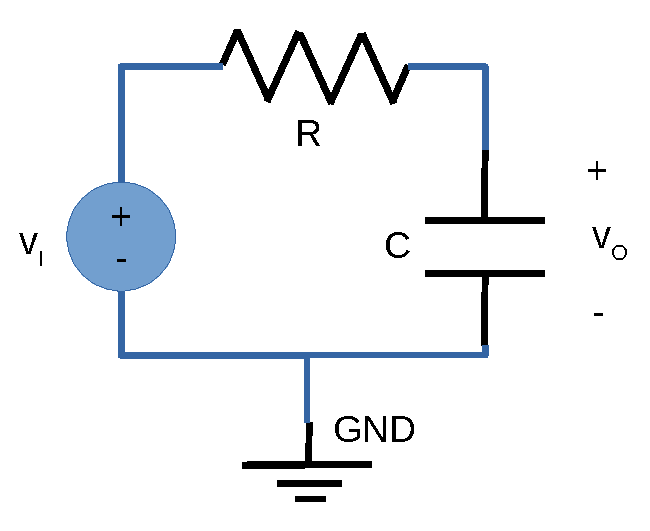
\includegraphics[width=0.65\linewidth]{rc.pdf}
\caption{AC/DC Converter}
\label{fig:rc}
\end{figure}
